	\section{Alfabeto}
	\subsection{Descripción del problema}
	El objetivo de esta practica es el generar las potencias del alfabeto binario $ \sum = \lbrace 0, 1 \rbrace $ desde $k=0$ hasta un $k$ seleccionado con un máximo de $k=1000$, para después guardar en un archivo todas las cadenas que se pudieron formar bajo estas condiciones, es decir: 
	\[{\sum}^{+} = {\sum}^{0}\cup{\sum}^{1}\cup{\sum}^{2}\cup\cdots\cup{\sum}^{1000}\]
	Es importante señalar que este conjunto solo es un subconjunto de $ {\sum}^{*} $ que representa todas las cadenas que se pueden formar con este alfabeto binario.
	El programa cuenta con modo manual (el usuario ingresa un $k$) y automático (genera su propio $k$).
	\subsection{Código}
	El código del programa fue realizado en C.
	\\Archivo: albafeto.h
	\begin{lstlisting}[language=C]
	//albafeto.h
	#ifndef __ALFABETO__
	#define __ALFABETO__
	
	#include <stdio.h>
	#include <stdlib.h>
	#include <time.h>
	
	static const int CONTINUAR = 1;
	int iniciar();
	int abrir_archivo(FILE **);
	int generar_palabras();
	
	#endif
	\end{lstlisting}
	Archivo: alfabeto.c
	\lstset{language=C}
	\begin{lstlisting}
	//alfabeto.c
	#include "alfabeto.h"
	
	int generar_palabras(int potencia_k) {
		FILE *archivo = NULL;
		int long_cadena;
		int i;
		int posicion;
		int *cadena_aux = NULL;
		
		abrir_archivo(&archivo);
		fputs("S = {e", archivo);
		
		for (long_cadena = 1; long_cadena <= potencia_k; long_cadena++) {
			cadena_aux = (int*) calloc(long_cadena, sizeof(int));
			if(cadena_aux == NULL) {
				printf("%s\n", "Error en el calloc");
				exit(0);
			}
			while(CONTINUAR) {
				fputc(',', archivo);
				for(i = 0; i < long_cadena; i++) {
					fputc(cadena_aux[i] + '0', archivo);
				}
				for(posicion = 0; posicion < long_cadena; posicion++) {
					cadena_aux[posicion] += 1;
					if(cadena_aux[posicion] > 1) {
						cadena_aux[posicion] = 0;
					} else {
						break;
					}
				}
				if(posicion >= long_cadena) {
					free(cadena_aux);
					break;
				}
			}
			printf("Va en 2^%d\n", long_cadena);
		}
		
		fputs("}", archivo);
		fclose(archivo);
		return 1;
	}
	
	int abrir_archivo(FILE **archivo) {
		*archivo = fopen("palabras.txt", "w");
		if (*archivo == NULL) {
			printf("%s\n", "No se pudo abrir");
			exit(0);
		}
		return 1;
	}
	
	\end{lstlisting}
	Archivo: main.c
	\begin{lstlisting}[language=C]
	//albafeto.h
	#include "main.c"
	
	int iniciar();
	int menu();
	int menu_continuar();
	int random_potencia_k();
	
	int main(int argc, char const *argv[]) {
		printf("%s\n", "***************Alfabeto****************");
		iniciar();
		return 0;
	}
	
	int iniciar() {
		srand(time(NULL));
		int continuar = 1;
		int potencia_k = 1;
		int manual = 1;
		while(continuar) {
			manual = menu();
			if (manual == 1) {
				printf("%s\n", "Ingresa el valor de k: ");
				scanf("%d", &potencia_k);
			} else if (manual == 2) {
				potencia_k = random_potencia_k();
			} else {
				break;
			}
			printf("El valor de k es: %d\n", potencia_k);
			generar_palabras(potencia_k);
			printf("%s\n", "Cadenas guardadas en el archivo palabras.txt");
			continuar = menu_continuar();
		}
		printf("\n%s\n", "Saliendo...");
		return 1;
	}
	
	int menu_continuar() {
		int opcion;
		printf("Intentar otra vez?\nSi = 1 NO = 0\n");
		scanf(" %d", &opcion);
		return opcion;
	}
	
	int menu() {
		int opcion;
		printf("Que quieres hacer?\n1.-Manual\n2.-Automatico\n3.-Salir\n");
		scanf(" %d", &opcion);
		return opcion;
	}
	
	int random_potencia_k() {
		//numero = rand () % (N-M+1) + M;
		// Cambiar el valor del random k a 1000
		int potencia_k = 1 + rand() % (1000 + 1 - 1);
		return potencia_k;
	}
	\end{lstlisting}
	\subsection{Pruebas}
	Las pruebas están divididas en modo automático y manual, en ambos dada una k se generan todas las cadenas de longitud 1 hasta $k$.
	\\\\
	{\large Modo automático.}
	\begin{figure}[H]
		\begin{center}
			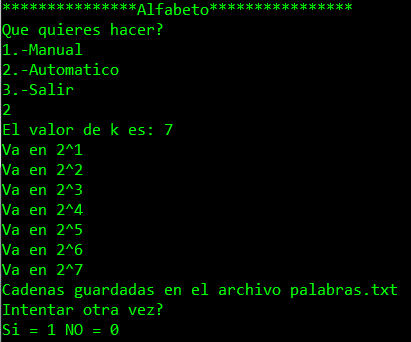
\includegraphics[width=7cm, height=7cm]{img/automatico-alfabeto.png}
			\caption{Alfabeto con k = 7.}
			\label{fig:alfabeto1}
		\end{center}
	\end{figure}
	\begin{figure}[H]
		\begin{center}
			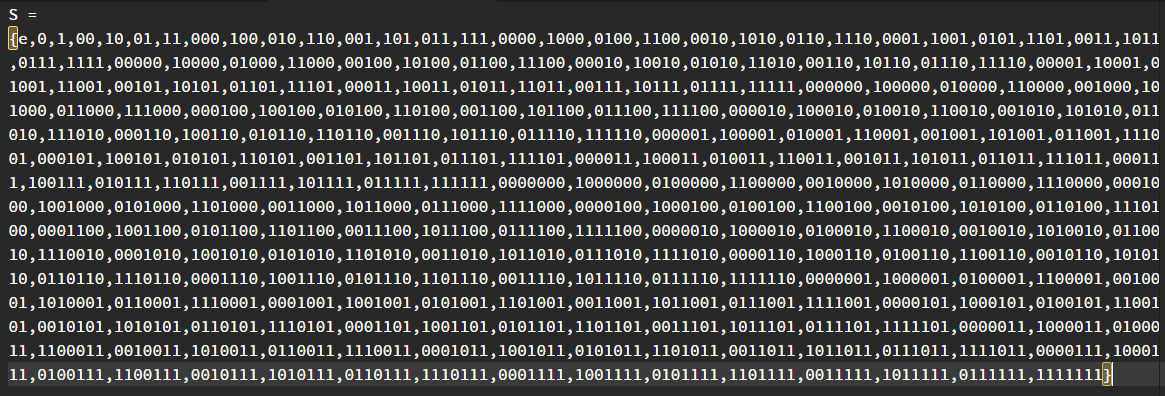
\includegraphics[width=\linewidth, height=8cm]{img/automatico-alfabeto-salida.png}
			\caption{Archivo generado.}
			\label{fig:alfabeto2}
		\end{center}
	\end{figure}
	{\large Modo manual.}
	\begin{figure}[H]
		\begin{center}
			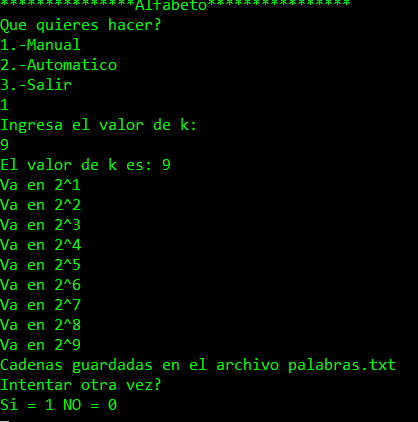
\includegraphics[width=7cm, height=7cm]{img/manual-alfabeto.png}
			\caption{Alfabeto con k = 9.}
			\label{fig:alfabeto3}
		\end{center}
	\end{figure}
	\begin{figure}[H]
		\begin{center}
			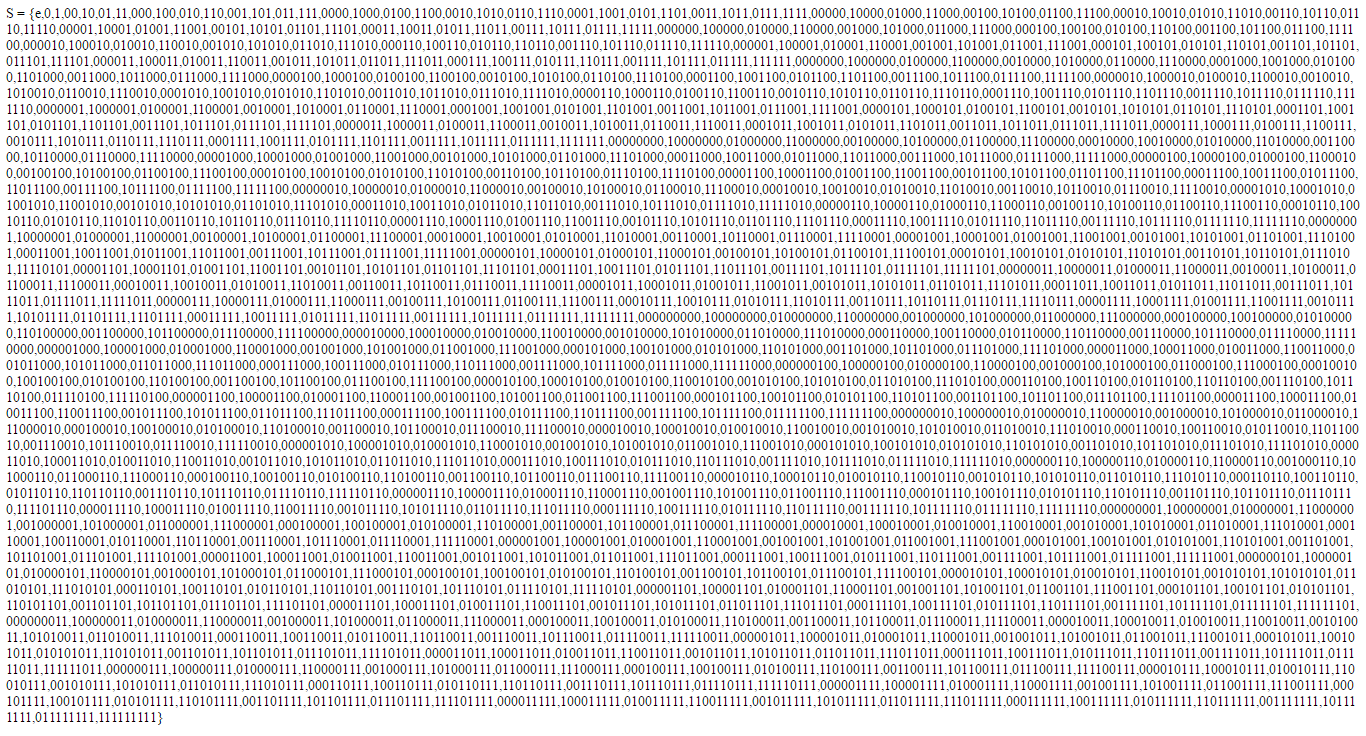
\includegraphics[width=\linewidth, height=12cm]{img/manual-alfabeto-salida.png}
			\caption{Archivo generado.}
			\label{fig:alfabeto4}
		\end{center}
	\end{figure}